%%----------------------------------------------------------------------------
%% Presentatie HoGent Bedrijf en Organisatie
%%----------------------------------------------------------------------------
%% Auteur: Bert Van Vreckem [bert.vanvreckem@hogent.be]

\documentclass{beamer}

%==============================================================================
% Aanloop
%==============================================================================

%---------- Packages ----------------------------------------------------------
\usepackage{etex}
\usepackage{graphicx,multicol}
\usepackage{comment,enumerate,hyperref}
\usepackage{amsmath,amsfonts,amssymb}
\usepackage{tikz}
\usepackage[dutch]{babel}
\usepackage[utf8]{inputenc}
\usepackage{multirow}
\usepackage{eurosym}
\usepackage{listings}
\usepackage[T1]{fontenc}
\usepackage{lmodern}
\usepackage{textcomp}
\usepackage{framed}
\usepackage{wrapfig}
\usepackage{pgf-pie}
\usepackage{pgfplots}
\usepackage{booktabs}
\usepackage{pgfplotstable}
\usepackage{changepage}
\usepackage{pst-plot,pst-func}

%---------- Configuratie ------------------------------------------------------

\usetikzlibrary{arrows,shapes,backgrounds,positioning,shadows}
\usetikzlibrary{pgfplots.statistics}


\usetheme{hogent}
\setbeameroption{show notes}

%---------- Commando-definities -----------------------------------------------

\newcommand{\tabitem}{~~\llap{\textbullet}~~}
\renewcommand{\arraystretch}{1.2}

%---------- Info over de presentatie ------------------------------------------

\title[Intro]{Onderzoekstechnieken\\$\chi^{2}$ toets}
\author{Jens Buysse \and Wim {De Bruyn} \and Wim Goedertier \and Bert {Van Vreckem}}
\date{AJ 2017-2018}

%==============================================================================
% Inhoud presentatie
%==============================================================================

\begin{document}

%---------- Front matter ------------------------------------------------------

% Dia met het HoGent logo
\HoGentLogo

% Titeldia met faculteitslogo
\titleframe

%---------- Inhoud ------------------------------------------------------------

\pgfmathdeclarefunction{gauss}{2}{%
  \pgfmathparse{1/(#2*sqrt(2*pi))*exp(-((x-#1)^2)/(2*#2^2))}%
}



\begin{frame}
  \frametitle{What's on the menu today?}

  \tableofcontents
\end{frame}

\begin{frame}
  \frametitle{Wat weten we nog van vorige les?}

  \begin{itemize}
    \item Wat is een hypothese
    \item Wat zijn de onderdelen van een hypothesetoets
    \item Wat zijn de stappen bij het toetsen?
    \item Welke fouten kunnen er gemaakt worden?
  \end{itemize}
\end{frame}

\section{$\chi^{2}$ toets voor een variabele}
\sectionframelogo{}

\begin{frame}
  \frametitle{Goodness of fit test}
  \brightbox{De \textcolor{HoGentAccent6}{goodness of fit test} kan gebruikt worden om na te gaan in welke mate de steekproef overeenstemt met een nulhypothese over de verdeling van de variabele.}

  \begin{columns}
    \begin{column} {0.5\textwidth}

    \begin{figure}
      \centering
        
\includegraphics[width=0.8\textwidth]{img/les6-man.jpg}
    \end{figure}

    \end{column}
    \begin{column} {0.5\textwidth}

    \begin{figure}
      \centering
        
\includegraphics[width=1.00\textwidth]{img/les5-heroes.jpg}
    \end{figure}

    \end{column}
  \end{columns}
\end{frame}

\begin{frame}
  \frametitle{Goodness of fit test}
   We willen  nagaan of de verdeling van onze steekproef bij $n = 400$ superhelden overeenstemt met de verdeling die je verwacht in de volledige populatie (de verzameling van alle mogelijke superhelden).


  \begin{itemize}
    \item We Vergelijken daartoe de aantallen in de steekproef met de aantallen die je zou verwachten als de steeproef exact representatief zou zijn naar de types van superhelden.
    \item Verschillen relatief groot $\Rightarrow$ dan komt de verdeling in de steekproef niet overeen
    \item Verschillen relatief klein $\Rightarrow$ dan komt de verdeling in de steekproef overeen
  \end{itemize}

  \pause
  Zie je een overeenkomst bij kruistabellen en Cramer's V?
\end{frame}

\begin{frame}
  \frametitle{Goodness of fit test}
  \begin{columns}
    \begin{column} {0.2 \textwidth}

    \begin{figure}
      \centering
        
\includegraphics[width=\textwidth]{img/les6-man.jpg}
    \end{figure}

    \end{column}

    \begin{column} { 0.8 \textwidth}
    \begin{table}[h]
\begin{tabular}{@{}lll@{}}
\toprule
\textbf{Type superheld} & \textbf{\# in steekproef} & \textbf{\# in populatie} \\ \midrule
Mutant                  & 127                       & 35\%                     \\
Mens                    & 75                        & 17\%                     \\
Alien                   & 98                        & 23\%                     \\
God                     & 27                        & 8\%                     \\
Demon                   & 73                        & 17\%                      \\ \bottomrule
\end{tabular}
\end{table}
    \end{column}
  \end{columns}
\end{frame}

\begin{frame}
  \frametitle{Goodness of fit test}
\begin{itemize}
  \item We willen kijken of de steekproef voor onze superhelden representatief is.
  \item Als de steekproef exact representatief is $\Rightarrow$ in steekproef 35\% van de superhelden een mutant
  \item Het verwachte aantal is dus gelijk aan $0.35 \times 400 = 140$.
  \item De verwachte frequenties worden genoteerd met de letter $e$ (expected).
\end{itemize}
 Er geldt dus:

\[ e = n \times \pi \]

Als de verschillen $o - e$  relatief klein zijn kunnen ze toegerekend worden aan toevallige steekproeffouten.
\end{frame}

\begin{frame}
  \frametitle{Goodness of fit test}
  Beschouw $\chi^{2}$:

\[ \chi^{2} = \sum_{i=1}^{n} \frac{(o_{i} - e_{i})^{2}}{e_{i}} \]

We merken op:
\begin{itemize}
  \item indien de verschillen klein zijn $\Rightarrow$ verdeling komt voldoende overeen
  \item indien de verschillen groot $\Rightarrow$ verdeling niet representatief
\end{itemize}

$\chi^{2}$ meet de mate van strijgdigheid van de gegevens met de nullhypothese
\end{frame}

\begin{frame}
  \frametitle{Goodness of fit test}
  \begin{columns}
    \begin{column} {0.2 \textwidth}

    \begin{figure}
      \centering
        
\includegraphics[width=\textwidth]{img/les6-man.jpg}
    \end{figure}

    \end{column}

    \begin{column} { 0.8 \textwidth}
      % Please add the following required packages to your document preamble:
% \usepackage{booktabs}
\begin{table}[h]
\begin{tabular}{@{}llllll@{}}
\toprule
\textbf{Type superheld} & \textbf{$o$} & \textbf{$\pi$} & \textbf{$e$} & \textbf{$o -e$} & \textbf{$\frac{(o-e)^{2}}{e}$} \\ \midrule
Mutant                  & 127          & 35\%           & 140          & -13             & 1.21                           \\
Mens                    & 75           & 17\%           & 68           & 7               & 0.72                           \\
Alien                   & 98           & 23\%           & 92           & 6               & 0.39                           \\
God                     & 27           & 8\%            & 32           & -5              & 0.78                           \\
Demon                   & 73           & 17\%           & 68           & 5               & 0.37                           \\ \bottomrule
\end{tabular}
\end{table}
    \end{column}
  \end{columns}
\end{frame}


\begin{frame}
  \frametitle{Goodness of fit test}

  \begin{itemize}
    \item De teststatistiek $\chi^{2}$ is verdeeld volgens de chi kwadraat verdeling.
    \item Kritieke grenswaarde $g$ bij de $\chi^{2}$ verdeling: hierbij speel het aantal vrijheidsgraden een rol ($df$). Er geldt:

\[ df = k -1 \]

met $k$ het aantal categorie\"en.
\item $df = 5-1 = 4$.
\item De kritieke waarden voor een gegeven significantieniveau $\alpha$ en vrijheidsgraden $df$ is opnieuw gegeven in tabel.
  \end{itemize}
In ons voorbeeld is $\chi^{2} = 3.47$ met grenswaarde $g = 9.49$ en besluiten we omdat $3.47 < 9.49$ de steekproef representatief is ($H_0$ wordt aanvaard).
\end{frame}

\subsection{Toetsingsprocedure goodness of fit test}

\begin{frame}
  \frametitle{Toetsingsprocedure goodness of fit test}
  \begin{enumerate}
  \item \textbf{Bepalen hypotheses}
    \begin{itemize}
      \item $H_{0}$: steekproef is representatief naar populatie
      \item $H_{1}$: steekproef is niet representatief naar populatie
    \end{itemize}
  \item \textbf{Bepalen $\alpha$ en $n$} : $\alpha = 0.05$ en $n = 400$.
  \item \textbf{Toetsingsgrootheid en waarde ervan in steekproef}:
  \[ \chi^{2} = \sum_{i=1}^{n} \frac{(o_{i} - e_{i})^{2}}{e_{i}} \]
  \item \textbf{Bereken en teken kritiek gebied}: de toets is altijd rechtszijdig. Is de toetsingsgrootheid kleiner dan kritieke grenswaarde verwerp $H_{0}$ niet, anders verwerp $H_{0}$ en aanvaard $H_{1}$.
\end{enumerate}
\end{frame}

\subsection{Voorbeeld}

\begin{frame}
  \frametitle{Voorbeeld gezinnen}
  Beschouw alle gezinnen met 5 kinderen in een bepaalde gemeenschap.
  \pause
  Met betrekking tot samenstelling zijn er 6 mogelijkheden.
\begin{enumerate}
  \item 5 jongens
  \item 4 jongens, 1 meisje
  \item 3 jongens, 2 meisjes
  \item 2 jongens, 3 meisjes
  \item 1 jongen, 4 meisjes
  \item 5 meisjes
\end{enumerate}
Het onderzoek bevat 1022 gezinnen met 5 kinderen
\begin{center}
Zijn de waargenomen aantallen in de 6 klassen representatief voor een populatie waar de kans om een jongen te krijgen = kans om een meisje te krijgen = 0.5?
\end{center}
\end{frame}

\begin{frame}
  \frametitle{Voorbeeld}
  \begin{table}[h]
\begin{tabular}{@{}llllllll@{}}
\toprule
i       & 0  & 1   & 2   & 3   & 4   & 5  &  \\ \midrule
$o_{i}$ & 58 & 149 & 305 & 303 & 162 & 45 &  \\ \bottomrule
\end{tabular}
\end{table}
\pause
Indien de veronderstelling waar is wordt de kans $\pi_{i}$ om $i$ jongens te krijgen bepaald door een binominaalvedeling met parameters $n=5$ en $p=0.5$.
Bv. De kans om 2 jongens te krijgen met 5 kinderen is gelijk aan :

\[ (0.5)^{2} \times (1-0.5)^{5-2} \times \binom{5}{2} \]

Algemeen geldt dus:

\[ \pi_{i} = \binom{5}{i}\times 0.5^{i} \times 0.5^{5-i} = \frac{5!}{i!(5-i)!}\times 0.5^{i} \]
\end{frame}

\begin{frame}
  \frametitle{Voorbeeld}
  \begin{table}[h]
\begin{tabular}{@{}llllllll@{}}
\toprule
$i$                         & 0        & 1        & 2        & 3        & 4       & 5       &         \\ \midrule
$o_i$                      & 58       & 149      & 305      & 303      & 162     & 45      & 1022    \\
$\pi_i$                      & 0.03    & 0.15    & 0.31    & 0.31  & 0.15 & 0.031 & 1       \\
$e_i$                      & 31.68   & 159.43  & 318.86  & 318.86  & 159.43 & 31.68  &         \\
$\frac{(o-e)^{2}}{e}$ & 21.86 & 0.68259  & 0.60   & 0.78  & 0.041 & 5.59 & 29.57 \\
$r_i$                      & 4.74   & -0.89 & -0.93 & -1.07106 & 0.22 & 2.40 &         \\ \bottomrule
\end{tabular}
\end{table}
\end{frame}

\begin{frame}
  \frametitle{Voorbeeld}
  \begin{enumerate}
  \item \textbf{Bepalen hypotheses}
    \begin{itemize}
      \item $H_{0}$: steekproef is representatief naar populatie
      \item $H_{1}$: steekproef is niet representatief naar populatie
    \end{itemize}
  \item \textbf{Bepalen $\alpha$ en $n$} : $\alpha = 0.01$ en $n = 1022$.
  \item \textbf{Toetsingsgrootheid en waarde ervan in steekproef}:
  \[ \chi^{2} = \sum_{i=1}^{n} \frac{(o_{i} - e_{i})^{2}}{e_{i}} = 29.5766 \]
  \item \textbf{Bereken en teken kritiek gebied}:  kritieke grens is $15.0863$. Onze toetsingsgrootheid ligt dus in het kritieke gebied dus verwerpen we $H_{0}$.
\end{enumerate}
\end{frame}

\subsection{Gestandaardiseerde residuen}
\begin{frame}
  \frametitle{Gestandaardiseerde residuen}
  \brightbox{De \textcolor{HoGentAccent6}{gestandaardiseerde residuen}  duiden aan welke klassen de grootste bijdrage leveren aan de waarde van de grootheid. }
  \[ r_{i} = \frac{O_{i} - n \pi_{i}}{\sqrt{n \pi_{i}(1-\pi_{i})}} \]

  \begin{itemize}
    \item Er geldt algemeen: waarden groter 2 of kleiner dan $-2$ zijn extreem.
  \end{itemize}
  We kunnen dus besluiten dat het aantal gezinnen waarin alle kinderen hetzelfde geslacht hebben groter mag worden genoemd dan verwacht.

\end{frame}

\begin{frame}
  \frametitle{Voowaarden}
   Om de toets te mogen toepassen dient aan de volgende voorwaarden te zijn voldaan (Regel van Cochran)
\begin{enumerate}
  \item Voor alle categorie\"en moet gelden dat de verwachte waarde $e$ groter is dan 1.
  \item In ten hoogste 20 \% van de categori\"en mag de verwachte waarde $e$ kleiner dan 5 zijn.
\end{enumerate}
\end{frame}

\section{$\chi^{2}$ toets voor twee variabelen}
\sectionframelogo{}

\begin{frame}
  \frametitle{$\chi^{2}$ toets voor twee variabelen}
  De Chi-kwadraattoets \index{$\chi^{2}$kwadraatkruistabeltoets} laat zich eenvoudig uitbreiden tot een onderzoeksontwerp met twee variabelen, met respectievelijk $r$ en $k$ niveaus.
\end{frame}

\begin{frame}
  \frametitle{Rokersonderzoek}
  In deze studie onderzochten Doll en Hill de relatie tussen roken en longkanker. Doll en Hill schreven in 1951 alle Britse huisartsen aan met het verzoek om gegevens over hun leeftijd en rookgedrag. Vervolgens hielden ze jarenlang de overlijdensberichten en de doodsoorzaak bij en herhaalden dit periodiek. De eerste uitkomsten, na circa vier jaar, zijn in de volgende tabel samengevat.

  \begin{table}[h]
    \begin{tabular}{@{}lllll@{}}
      \toprule
                     & \textbf{Longkanker} & \textbf{Niet} & \textbf{Wel} & \textbf{Totaal} \\ \midrule
      \textbf{Roker} & \textbf{Wel}        & 21178         & 83           & 21261           \\
                     & \textbf{Niet}       & 3092          & 1            & 3093            \\
                     & \textbf{Totaal}     & 24270         & 84           & 24354           \\ \bottomrule
    \end{tabular}
  \end{table}
\end{frame}

\begin{frame}
  \frametitle{Rokersonderzoek}
  \begin{table}[h]
\begin{tabular}{@{}lllll@{}}
\toprule
      & \textbf{Longkanker} & \textbf{Niet} & \textbf{Wel} & \textbf{Totaal} \\ \midrule
Roker & Wel                 & 21178         & 83           & 21261           \\
      & Niet                & 3092          & 1            & 3093            \\
      & Totaal              & 24270         & 84           & 24354           \\ \bottomrule
\end{tabular}
\end{table}

\begin{columns}
  \begin{column}{0.3 \textwidth}

  \begin{figure}
    \centering
      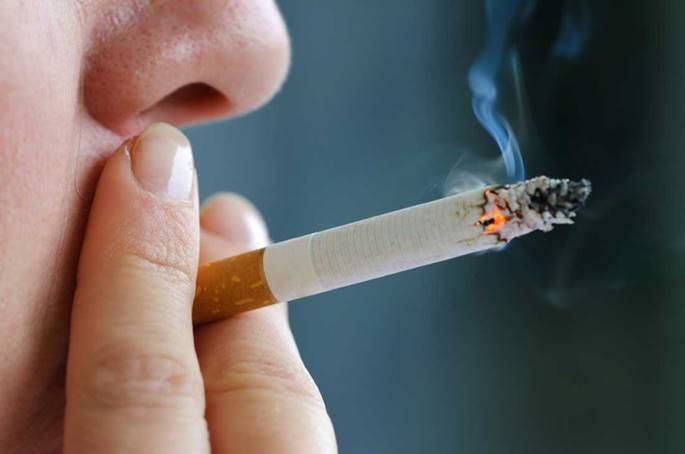
\includegraphics[width=1.00\textwidth]{img/les-6-smoking.jpg}
  \end{figure}

  \end{column}
  \begin{column}{0.7 \textwidth}

  \begin{itemize}
    \item \dots slechts $\frac{84}{ 24354} \times 100 = 0.35\% $ van de Britse artsen aan longkanker overleden
    \item \dots met slechts $\frac{83}{21261} \times 100 = 0.39\%$ van de rokers onder hen
    \item \dots maar  is wel  meer dan hetzelfde cijfer voor de niet-rokers $\frac{1}{3093} * 100 = 0.032\%$.
  \end{itemize}
  \end{column}
\end{columns}
\end{frame}

\begin{frame}
  \frametitle{Rokersonderzoek}
  % Please add the following required packages to your document preamble:
% \usepackage{booktabs}
\begin{table}[h]
\begin{tabular}{@{}lllll@{}}
\toprule
      & \textbf{Longkanker} & \textbf{Niet} & \textbf{Wel} & \textbf{Totaal} \\ \midrule
Roker & Wel                 & 21188         & 73.3         & 21261           \\
      & Niet                & 3082.3        & 10.7         & 3093            \\
      & Totaal              & 24270         & 84           & 24354           \\ \bottomrule
\end{tabular}
\end{table}

\begin{columns}
  \begin{column}{0.3 \textwidth}

  \begin{figure}
    \centering
      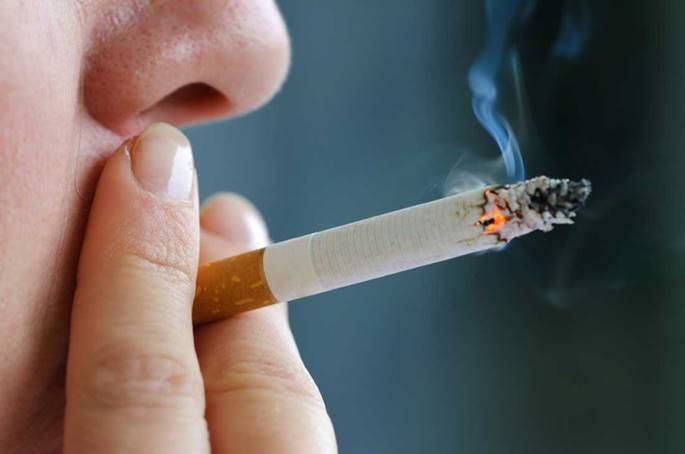
\includegraphics[width=1.00\textwidth]{img/les-6-smoking.jpg}
  \end{figure}

  \end{column}
  \begin{column}{0.7 \textwidth}

  \begin{itemize}
    \item $\chi^{2} = 10.35$
    \item We zien in de tabel  dat er wel een erg groot verschil is tussen de geobserveerde aantallen rokers die overlijden aan longkanker en de verwachte waarden in deze cel.
    \item Hetzelfde geldt voor het geringe aantal huisartsen dat niet rookt, maar wel aan longkanker overleden is.
  \end{itemize}
  \end{column}
\end{columns}
\end{frame}

\begin{frame}
  \frametitle{Rokersonderzoek}
  \begin{enumerate}
  \item \textbf{Bepalen hypotheses}
    \begin{itemize}
      \item $H_{0}$: in de populatie is er geen samenhang tussen onafhankelijke en afhankelijke variabele
      \item $H_{1}$: er bestaat wel een samenhang tussen de variabelen in de populatie
    \end{itemize}
  \item \textbf{Bepalen $\alpha$ en $n$} : $\alpha = 0.05$ en $n = 24354$.
  \item \textbf{Toetsingsgrootheid en waarde ervan in steekproef}:
  \[ \chi^{2} = \sum_{i=1}^{n} \frac{(o_{i} - e_{i})^{2}}{E_{i}} = 10.35 \]
  \item \textbf{Bereken en teken kritiek gebied}:  kritieke grens is 3.8415 en aantal vrijheidsgraden $df = (r-1)(k-1)$ Onze toetsingsgrootheid ligt dus in het kritieke gebied dus verwerpen we $H_{0}$.
\end{enumerate}
\end{frame}

\begin{frame}
  \frametitle{Oorzakelijk verband}
  We moeten derhalve $H_{0}$, dat er geen relatie is tussen beide variabelen, verwerpen ten gunste van $H_{1}$ dat er wel een relatie is tussen beide variabelen: rokers sterven vaker aan longkanker dan niet-rokers.
  \begin{columns}
  \begin{column}{0.3 \textwidth}

  \begin{figure}
    \centering
      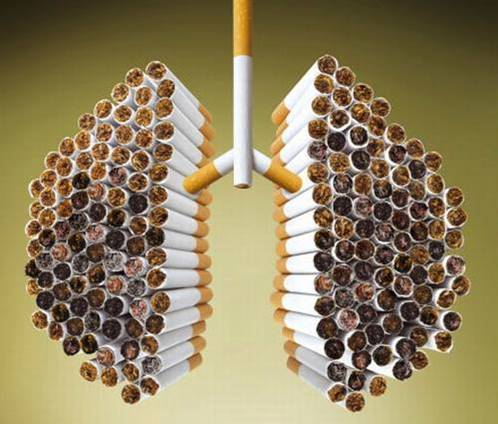
\includegraphics[width=1.00\textwidth]{img/les-6-smoking2.jpg}
  \end{figure}

  \end{column}
  \begin{column}{0.7 \textwidth}

  \begin{itemize}
    \item  \dots rokers zijn ouder dan de niet-rokers
    \item \dots de rokers wonen veelal in de grote steden met
meer vervuilde lucht dan de niet-rokers
    \item \dots speciale genetische dispositie die zowel van invloed is op de verslaving aan tabak, als op de kans om longkanker te krijgen.
  \end{itemize}
  \end{column}
\end{columns}
Voor een causale interpretatie van de gegevens (het betreft hier immers geen experiment), moeten we op zijn minst de beschikking hebben over een theorie die de relatie tussen roken en longkanker expliciteert.

\end{frame}

\end{document}
